%\section{Schedule and Cost Baseline}
\label{sec:schcost}

Cost estimates for engineering, designing, fabricating, assembling, testing, and installing the Heavy Photon Search detector are given below. The costs reflect considerable savings coming from the reuse of many parts of the Test Run, which was already made from the donation of the silicon microstrip sensors from Fermilab, the use of some DAQ crates and equipment from SLAC, and many contributions from JLab, including PbWO$_4$ calorimeter crystals, the chicane and analyzing magnets, magnet power supplies, and beam diagnostic apparatus. Much of the calorimeter readout electronics utilizes designs which are already in place for the Hall B 12 GeV upgrade, eliminating engineering and design expense. The SVT DAQ benefits from SLAC�s development of an ATCA readout system, and incorporates many of its designs. Very significant cost savings come from utilizing the FADCs and data acquisition system being developed for the upgraded CLAS12 detector, which will be available to the Test Run. The Orsay group is contributing engineering and design efforts for the ECal and its vacuum chamber, affording additional savings. 

The costs are given in an accompanying WBS summary table, below, which itemizes the major items subsystem by subsystem, and indicates whether JLab (J) or SLAC (S) takes responsibility for construction. Engineering, design, and technician labor rates include lab overheads, and differ between the two laboratories. Contingencies have been set at 20\%. The cost estimates are based on the experience of the real costs incurred for the construction and installation of the HPS Test Run Experiment. Our DAQ and beamline cost estimates have been made by engineering groups at SLAC and JLab which are experienced in cost estimation and actively involved in many related projects. The SVT estimates came from physicists and engineers on the project, with experience in designing and fabricating silicon detector systems. The Ecal estimates come from physicists and engineers at JLab and Orsay who have constructed a similar system, the CLAS IC, in the recent past. 

The schedule for the overall project is included in a Project Summary table below. A brief description of the schedule for the different subsystems is also given. The overall schedule contingency is about 20\%, and depends critically on the assumption that funding is available by mid 2013.. The HPS has been organized into a Work Breakdown Structure (WBS) for purposes of planning, managing and reporting project activities. Work elements are defined to be consistent with discrete increments of project work. Project Management efforts are distributed throughout the project, including conceptual design and R\&D. The HPS has 18 WBS Level-2 elements: 

\begin{table}[htdp]
\caption{Project WBS structure.}
\begin{center}
\begin{tabular}{|c|c|}
\hline
WBS& NAME \\
\hline\hline
1.1 & Beamline \\
\hline
1.2 & SVT \\
\hline
1.3 & SVT DAQ \\
\hline
1.4 & ECAL \\
\hline
1.5 & Muon \\
\hline
1.6 & TDAQ \\
\hline
1.7 & Slow Controls \\
\hline
1.8 & Installation \& Commissioning \\
\hline
1.9 & 2014 Commissioning Run \\
\hline
1.10 & SLAC Travel \\
\hline
1.11 & SLAC Travel 2015 Data Run \\
1.12 & Project Management  \\
\hline
\hline
\end{tabular}
\end{center}
\label{tb:wbs}
\end{table}%

\subsection{Cost}

The costs include Labor and M\&S. The labor is accounted only if provided by professional centers (engineering) at SLAC or JLAB and it does not include labor provided by physicists which is a dominant contribution to the  project. Labor rates have been applied following the official shop rates at SLAC and JLAB, which include already ~31\% fringe benefits. M\&S have been calculated by the best estimation of the commercially available parts and based on the real cost incurred for the TEST RUN. The overheads have been added to both labor and M\&S being respectively 53\% and 7.65\% at SLAC, 57.15\% and 49\% at JLAB. SLAC travel includes 53\% overheads. A uniform cost contingency of 20\% has been applied. Since the project is stage over three years, an annual inflation rate of 2.5\%  included in the FY14 and FY15 costs.

Beamline expenses for HPS are held to a minimum by using the 18D36 magnet currently installed in Hall B as the analyzing magnet, the two JLab Frascati chicane magnets and the Test Run vacuum box with the SVT vacuum box.  Some overall engineering and design will be required, beam pipes fabricated, the Muon System vacuum chamber designed and built, , a vacuum chamber built for the downstream Frascati magnet, and a photon dump and shielding inserted behind the second chicane magnet. Total beamline expenses are about \$300k.

Three out of the five planes of the SVT Test Run will be reused after modification of their supports which will provide improved mechanical stability and better cooling.. Three new planes with double sensors and their supports will be designed and built from scratch. Fermilab will donate the needed silicon microstrip detectors, as it had for the HPS Test Run. The tracker/vertexer for the test run will cost about \$590k.

The SVT DAQ requires small modifications to the  hybrid, readout  and flange board engineering design,prototyping, and production,, APV25 and chip procurement, and  fabrication and testing. The SVT DAQ also requires designing and prototyping the Trigger Interrupt ACTA card and new firmware for the APV25 to provide event buffering to accommodate higher trigger rates.. ATCA crates, and standard RCE cards are also required.. The expenses are dominated by engineering development, and total \$610k.  

JLab will donate the PbWO$_4$ crystals used in the ECal. Orsay will donate engineering and design for a new enclosure for the crystals, but Jlab will need to fabricate the enclosure, the crystal support structure, the readout motherboard and connection board, and support fixtures. It will also make repairs to the existing motherboards and acquire new power supplies. The total expense will be roughly \$270k, including fabrication, assembly, and testing.. Trigger and DAQ electronics for the ECAL are being developed for the CLAS upgrade, so relatively little engineering and technician time will be needed in preparation of the HPS Test Run except for providing special purpose firmware.. Components, including the 250 MHz FADC boards and crates will be provided at no cost since they can be borrowed from the CLAS upgrade. The system test expenses will also be borne by JLab Hall B. The total cost is \$300k. 

The Muon system costs are in purchasing  photomultipliers and scintillator, designing and fabricating  the absorbers and Muon System vacuum chamber, and building support stands and providing cables.The total is \$270k. 

The Slow Control is needed to monitor the operations of the three sub-detectors. In addition, they will control and interlock the movements of the SVT respect the beamline and provide beam protection interlocks.. The total cost is \$200K being essentially labor required to integrate the HPS with the existing Slow Control system in the Hall-B.

Travel and lodging expenses for SLAC trips to JLab are also included in this proposal. During design and construction, there will be a small number of trips to solidify and review designs, and to work together to begin DAQ integration of the SLAC and JLab systems. Funds are reserved for a collaboration meetings to be held during calendar 2013 and 2014 at JLab. Funds are also reserved  to staff installation, commissioning, and data taking runs. The total is \$190K.

{\bf The total cost for HPS is \$2.8 M. }

HPS is seeking funding from other sources for the Muon System and the Ecal.
William\&Mary will submit an MRI proposal to NSF for the Muon System, requesting $\sim \$130$k. IPN ORSAY (France) has submitted a proposal to a French funding agency for the ECal  Light Monitoring System (\$100k) and for a new, high performance  APD�s to improve crystal readout (\$500k) and other expenses related to ECal fabrication and test test. Note that the new APDs are not part of this proposal. If the requests are approved the corresponding funding will be subtracted from the total cost of the HPS. 

\subsection{Schedule}

Our goal is to be ready to install the HPS in Hall-B at JLAB  by September 2014, and proceed with the commissioning on beam with the CEBAF early physics beam window opportunity in October 2014. The data taking will continue in 2015 until Summer.. Meeting this schedule  will require approval and funding as soon as possible, preferably by June 2013.. Schedules for each of the major subsystems of the experiment are attached below, and summarized here. The total construction schedule extends over  16 months, assuming the funding available mid-2013. The schedule contingency is about 20\%. 

The conceptual design of the beamline will be done during 2013. Formal beamline engineering will start when funding is secured.  A Beamline Engineering Design Review will be held in February 2014 to validate the concept before the start the major spending. Final Engineering and Construction will start in Spring 2014 and end well before the installation time in October 2014, wlproviding substantial float. Using keep-alive funds, the Test Run SVT will be shipped back to SLAC by early February 2013 to rework the modules for the first three layers of the HPS and commission the motion control systems.. The conceptual design of the Layers 1-2-3 and Layers 4-5-6 will start already in spring 2013 using keep alive funding.. An Engineering Design Review of the SVT will be held in November 2013, after the funding has been released and before the final production. Preliminary engineering for the SVT DAQ is already underway, using the same keep alive funds. The SVT DAQ will formally begin work in  the second half 2013, after funding and an Engineering Review. The assembly and integration test at SLAC are expected in Spring 2014 and the SVT will be ready for shipping on July 2014. The SVT will be ready for tinstallation at mid-august 2014. SVT  installation in the analyzing magnet vacuum chamber will occur inSeptember, depending on the schedule of the Hall-B.  The SVT schedule has 1 month of float between the shipping and the test at JLAB, which will be eventually used as contingency for  construction work at SLAC.

The Ecal work will start in the second half 2013 and run through June 2014. The ECAL will be ready for installation by June 2014. The Muon System work will start in July 2013 with a design phase which will be validated in an Engineering Design Review in September 2013. It will be ready for installation on August 2014, with one month of float with respect to  the installation date.
The schedule includes seven milestones to track the progress of each subssytem. They will monitor the subdetector readiness after testing at the respective assembly sites, and the readiness for installation at JLAB.  Also, ad-hoc Engineering Design Reviews will be called by the PM for each subsystem before major costs are incurred.

\begin{table}[htdp]
\caption{Project Milestones.}
\begin{center}
\begin{tabular}{|c|c|c|}
\hline
WBS & Milestones & Date\\
\hline\hline
1.1.21&Beamline Installation&26-Sep-14 \\
\hline
1.2.1	&SVT returns from JLAB	&18-Feb-13 \\
\hline
1.2.12&	SVT Shipped at JLAB	&16-Jun-14\\
\hline
1.2.14&	SVT Ready For Installation&	15-Aug-14\\
\hline
1.4.12&	ECAL Ready for the installation&	8-Aug-14\\
\hline
1.5.9	&Muon Ready for installation&	30-May-14\\
\hline
1.10.7&	HPS ready for the beam&	12-Sep-14\\
\hline
\hline
\end{tabular}
\end{center}
\label{tb:milestones}
\end{table}%

\begin{table}[htdp]
\caption{Planned Review.}
\begin{center}
\begin{tabular}{|c|c|c|}
\hline
WBS&Engineering Reviews& Data\\
\hline
\hline
1.1.2 &	Beamline  Review&	3-Feb-14\\
\hline
1.2.2	&SVT Design Review	&14-Oct-13\\
\hline
1.5.1	&Muon Design Review&	2-Sep-13\\
\hline
1.10.1&	Installation Review	&21-Jul-14\\
\hline
\hline
\end{tabular}
\end{center}
\label{tb:reviews}
\end{table}%

\subsection{Manpower}

The manpower needed to design, fabricate, assemble, test, install, and commission the HPS is captured in the WBS tables. The HPS Collaboration has the personnel needed to realize this project. 
Beamline design work will be done at JLab by Arne Freyberger and Stepan Stepanyan and at SLAC by Ken Moffeit; engineering at SLAC by Marco Oriunno, Dieter Walz, and Clive Field; fabrication in the JLab shops; and installation by the Hall B crew. 

Engineering for the Ecal is being done by Philippe Rosier at Orsay in consultation with Marco Oriunno. 

Beam diagnostics and slow control will be supported by Nerses Gevorgyan (Yerevan) and Hovanes Egiyan.

 
The Tracker/Vertexer will be engineered and designed by Marco Oriunno, Tim Nelson and Per Hansson, with additional help from Vitaly Fadeyev,Alex Grillo, and Bill Cooper,, all experienced with silicon detector systems. Others at SLAC and UCSC will help with test and assembly, including Matt Graham, Takashi Maruyama, John Jaros,, a post doc, and graduate students Sho Uemura and Omar Moreno.  Matt McCulloch will serve as the  technician at SLAC. 

The Ecal is being designed by the Orsay Group, especially Philippe Rosier, Emmanuel Rindel, Emmanuel Rauly, Raphael Dupre, and Michel Guidal, with participation by the Jlab group, especially Stepan Stepanyan, and F.-X. Girod. Others at JLab and in the collaboration will help in assembly and test of the ECal, especially groups from Norfolk State University (Carlos Salgado), and INFN Genova(Italy). 
 
The SVT DAQ is being done by Haller�s group at SLAC, including Gunther Haller, Ryan Herbst, Tung Phan, and Raghuveer Ausoori. SVT Physicists Per Hanssen, Alex Grillo, Vitaliy Fadeyev, and Tim Nelson will collaborate closely. Postdocs and students will help debug, test, and certify DAQ electronics. 

The Ecal Trigger/DAQ work is done in Sergey Boyarinov�s group, which supports Hall B activities at JLAB, and with Chris Cuevas� group, which has designed the FADC250. R. Dupre and V. Kubarovsky will collaborate with this group in assembling and testing the electronics, programming the trigger, and integrating it with the Ecal hardware.

 The HPS collaboration is nearly 60 strong, so has adequate manpower for overall installation, commissioning, and data taking.  Simulation work is supported by Maurik Holtrop, Matt Graham, M.Ungaro, and Takashi Maruyama, along with help from students and Norman Graf  and Jeremy McCormiock at SLAC. Data management and storage and computing infrastructure will be overseen by Sergey Boyarinov and Maurik Holtrop and Homer Neal, all very experienced professionals. Analysis and simulation studies have been initiated by Maurik Holtrop, Matt Graham, and Takashi Maruyama. Students are actively being engaged. 
The HPS collaboration is managed by its three spokespersons, Maurik Holtrop, John Jaros, and Stepan Stepanyan and its Executive Committee, which consists of the spokespeople along with Takashi Maruyama, Matt Graham, Tim Nelson, and F-X Girod . Ten working groups supervise the progress of each sub-system. The Project Manager is Marco Oriunno.

\begin{table}[htdp]
\caption{Working groups.}
\begin{center}
\begin{tabular}{|c|c|c|}
\hline
HPS working Groups	& Chair (Deputy)\\
\hline\hline
Beamline	&K. Moffeit (FX Girod)\\
\hline
SVT	&T.Neslon (V.Fedayev)\\
\hline
ECAL	& R. Dupre (S.Stepanyan)\\
\hline
DAQ	 & S. Boiarinov (P.Hansson)\\
\hline
Trigger &	V. Kubarovsky (T.Maruyama)\\
\hline
Slow Control	& H. Egiyan (N. Gevorgyan)\\
\hline
Muon &	K.Griffioen (Y.Gershtein)\\
\hline
Software	& M.Haltrop (S. Uemura)\\
\hline
Analysis &	M. Graham (O. Moreno)\\
\hline
Project Management &	M. Oriunno (S. Stepanyan, J.Jaros)\\
\hline
\end{tabular}
\end{center}
\label{tb:groups}
\end{table}%

\begin{table}[htdp]
\caption{Distribution of resources.}
\begin{center}
\begin{tabular}{c|ccc}
Res.	 &SLAC	&JLAB	&ORSAY\\
\hline\hline
ME	&1,513	&194	&0 \\
MD	&720	&750	&0\\
MT	&1,130	&420	&40\\
EE 	&2,400	&2,352&	800\\
\end{tabular}
\end{center}
\label{tb:resources}
\end{table}%

\begin{table}[htdp]
\caption{Total Engineering Labor (hrs) required for three years. Only SLAC and JLAB charge costs.}
\begin{center}
\begin{tabular}{c|cccc}
 FTE	&FY13	&FY14	&FY15&	TOT\\
 \hline\hline
ME	&0.42	&0.44&	0.00&	0.86\\
MD&	0.31	&0.10&	0.00&	0.41\\
MT&	0.41	&0.24&	0.00	&0.64\\
EE &	1.16	&0.20&	0.00	&1.36\\
ET&	0.02	&0.00&	0.00	&0.02\\
Physicist	&4.22	&3.92	&4.15	&12.24\\
\end{tabular}
\end{center}
\label{tb:engin}
\end{table}%

{\bf {\large Cost Breakdown HPS}

\begin{figure*}[h]
\centering
%\vspace*{-5mm}
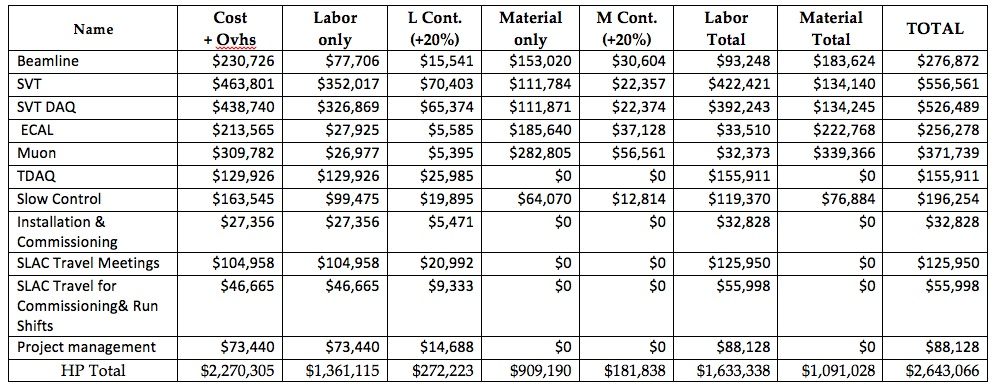
\includegraphics[angle=90,width=0.6\textwidth]{cost_schedule/cost_systems_table.jpg} 
\caption{Cost breakdown by sub-systems.}
\label{fig:cost}
\end{figure*}

\begin{figure*}[h]
\centering
%\vspace*{-5mm}
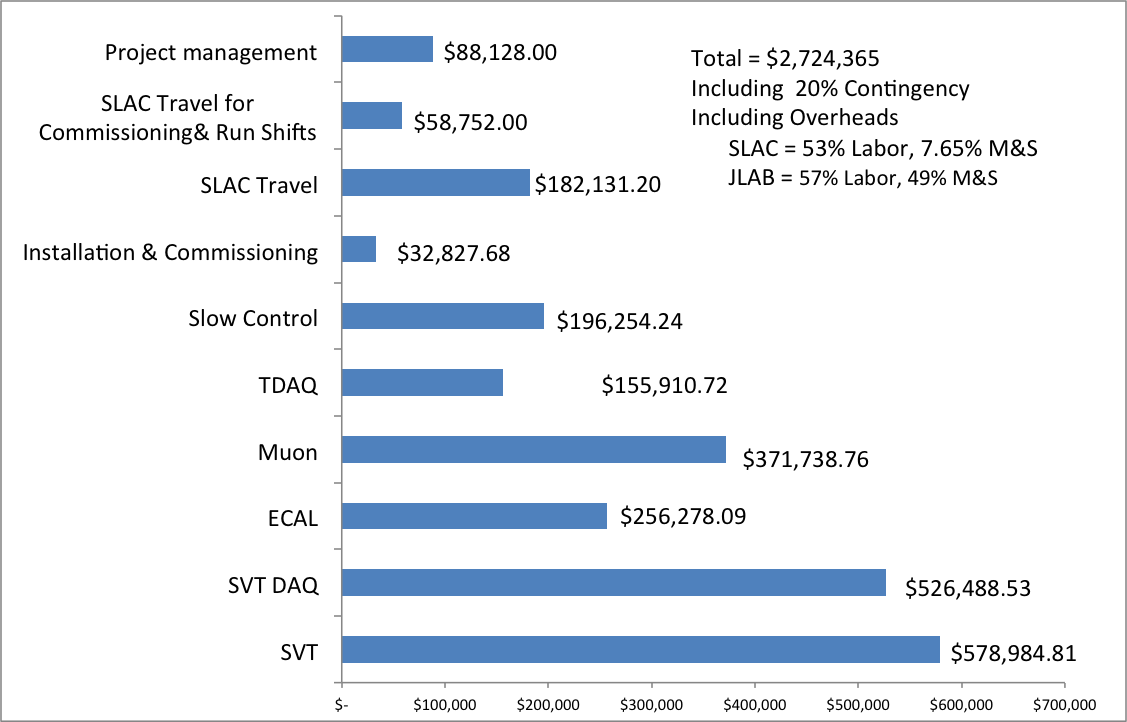
\includegraphics[width=0.9\textwidth]{cost_schedule/cost_systems.jpg} 
\caption{Cost breakdown by sub-systems.}
\label{fig:cost}
\end{figure*}

\begin{figure*}[h]
\centering
%\vspace*{-5mm}
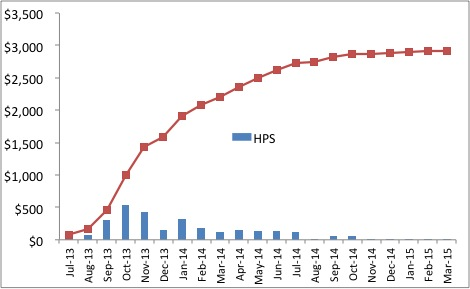
\includegraphics[width=0.9\textwidth]{cost_schedule/spending.jpg} 
\caption{Spending profile (costs after overheads and contingency).}
\label{fig:spending}
\end{figure*}

\begin{figure*}[h]
\centering
%\vspace*{-5mm}
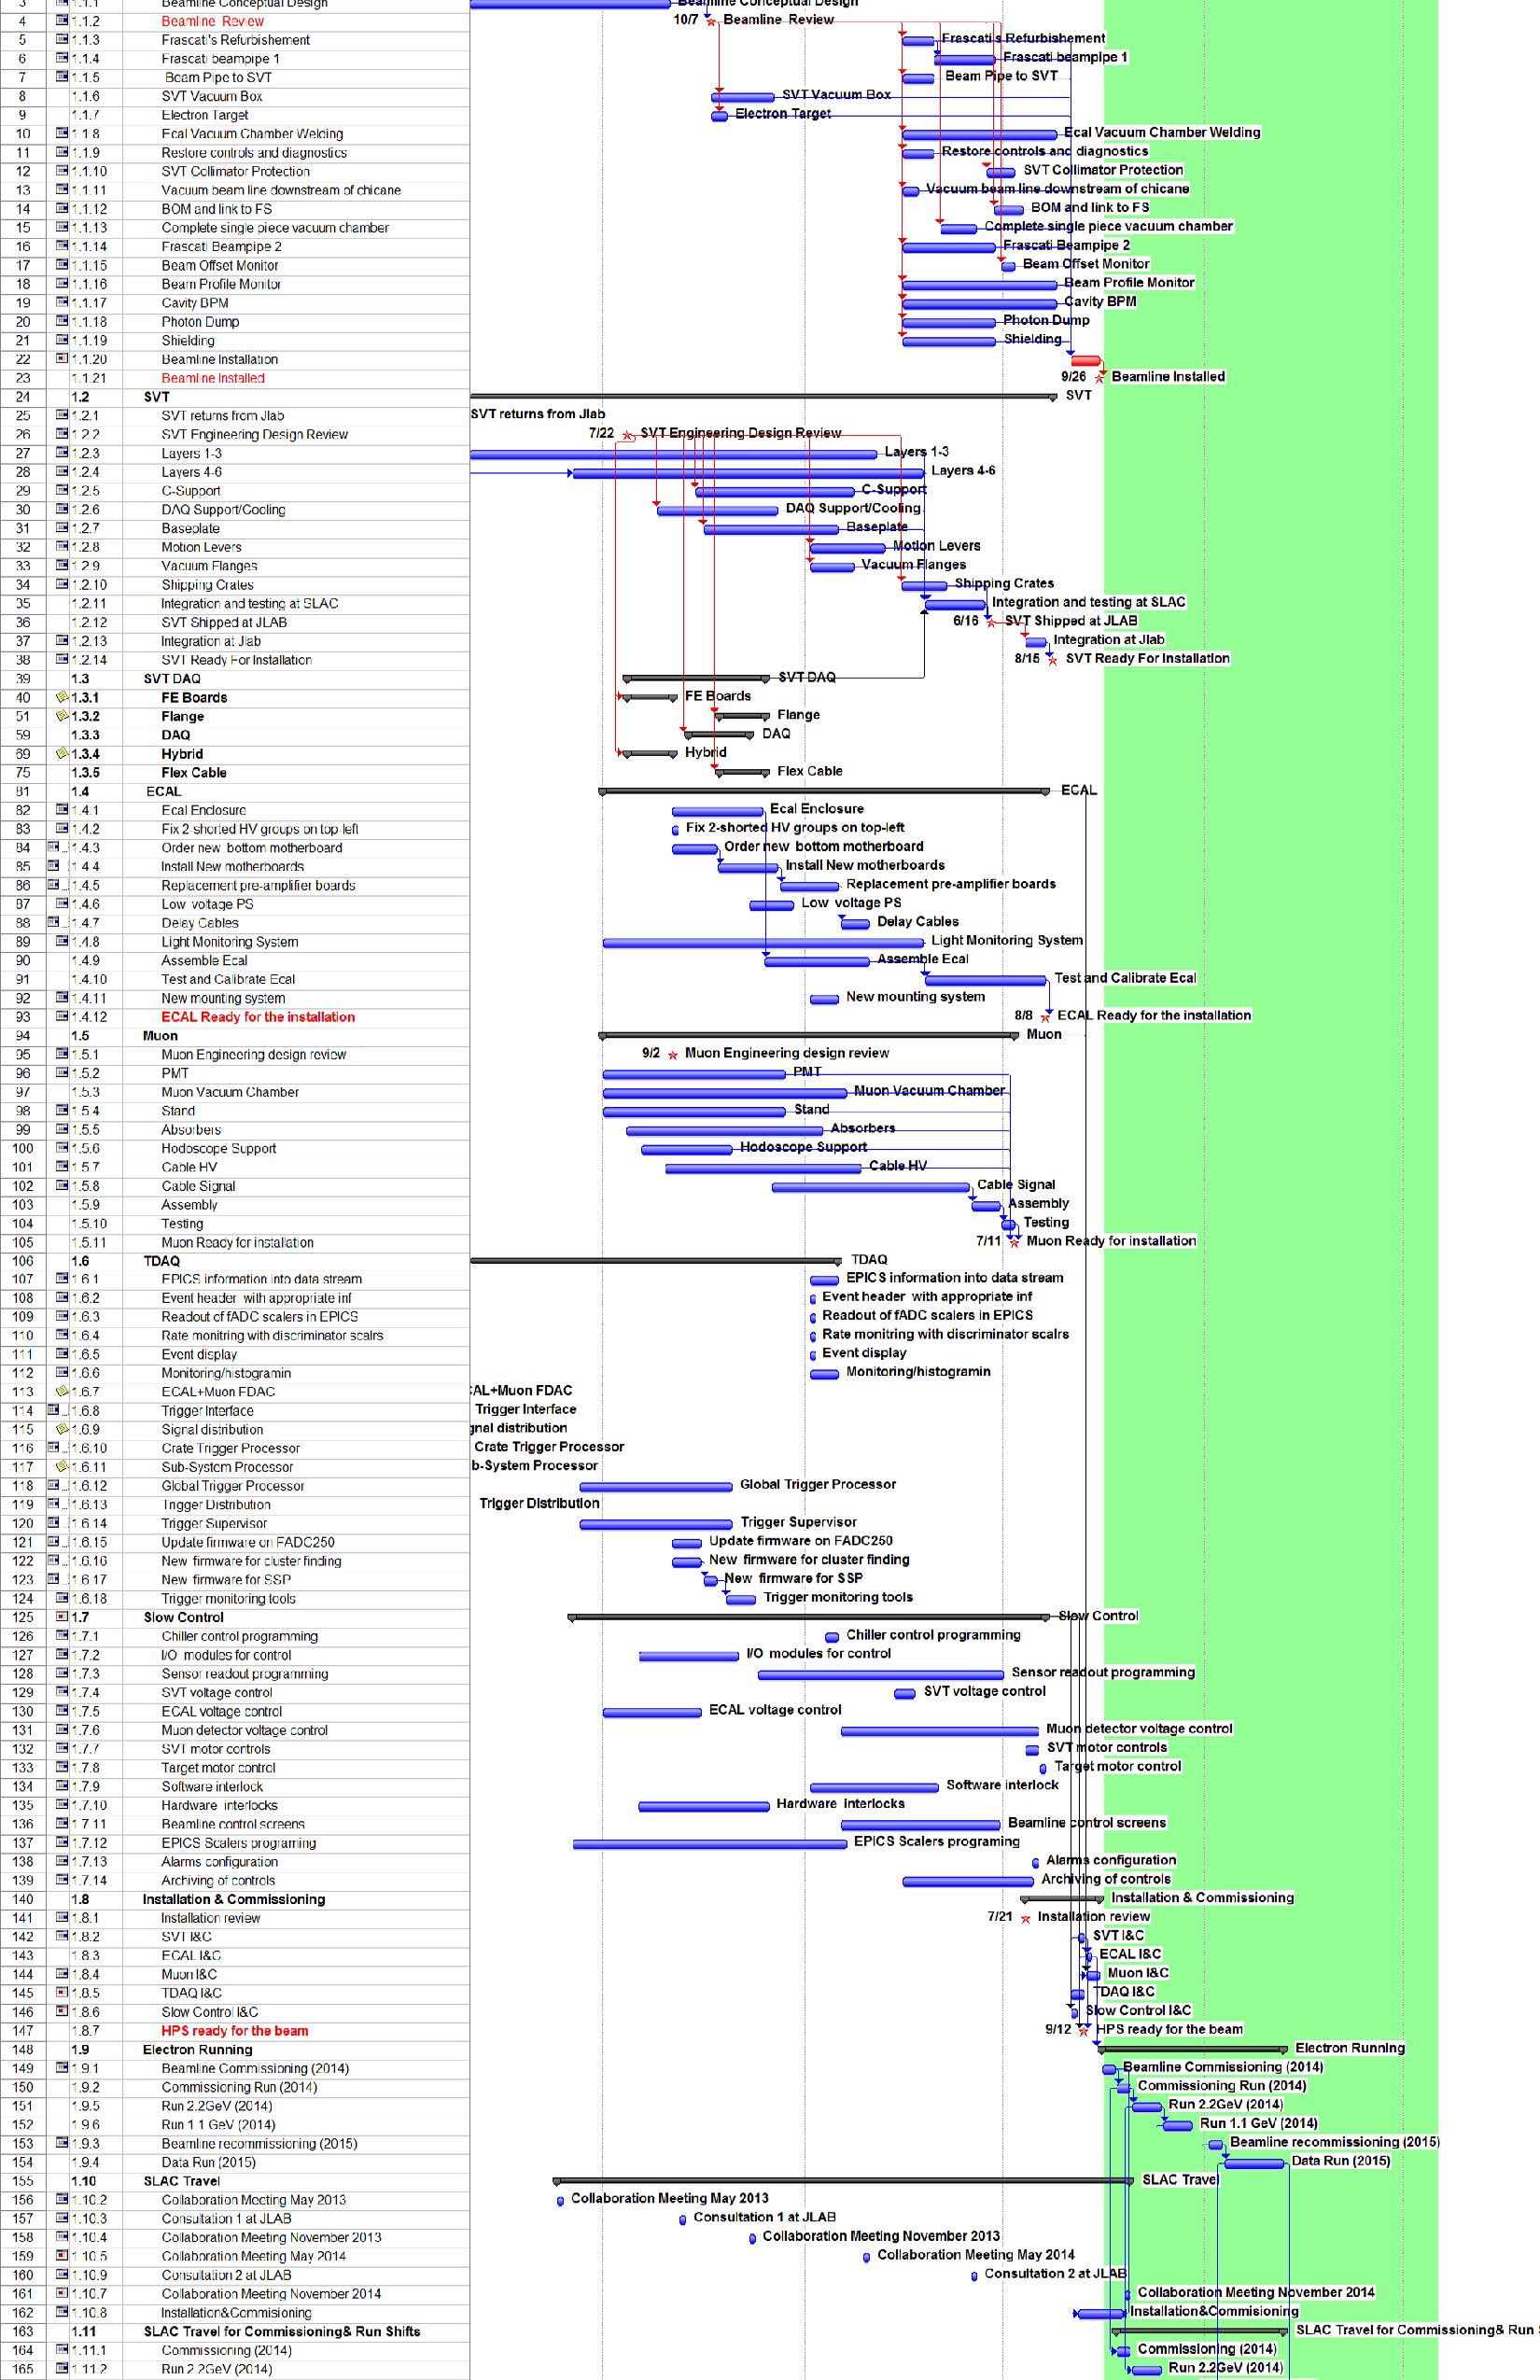
\includegraphics[angle=0,width=0.85\textwidth]{cost_schedule/HPSV70} 
\caption{HPS schedule.}
\label{fig:schedulea}
\end{figure*}


